\documentclass[11pt,a4paper]{article}
\usepackage[T1]{fontenc}
\usepackage[utf8]{inputenc}
\usepackage{lmodern,microtype}
\usepackage[margin=25mm]{geometry}
\usepackage{graphicx,booktabs,tabularx,array,xcolor}
\usepackage[hidelinks]{hyperref}
\setlength{\emergencystretch}{2em}
\setlength{\parskip}{5pt}
\setlength{\parindent}{0pt}
\setcounter{tocdepth}{1}
\graphicspath{{figures/}}
\begin{document}\hypersetup{pageanchor=false}
\begin{titlepage}\centering
\vspace*{28mm}
{\Large Human Computer Interaction\par}
\vspace{16mm}
{\Huge\bfseries A11yNav\par}
\vspace{7mm}
{\LARGE An AI-Powered Guided\\[3mm] Navigation Assistant\par}
\vspace{12mm}
{\large Experimental Project Report\par}
\vspace{23mm}
\begin{tabular}{lr}\toprule
\textbf{Team member} & \textbf{ERP}\\\midrule
Azhab Safwan Babar & 29227\\[3mm]
Gaurav Khatwani & 29213\\[3mm]
Ibrahim Irfan Nazar & 29225\\\bottomrule
\end{tabular}
\vfill
\textbf{GitHub repository}\\[3mm]
\url{https://github.com/Ibrahim-1rfan/A11yNav}
\vspace{14mm}\end{titlepage}
\pagenumbering{roman}\hypersetup{pageanchor=true}\tableofcontents\clearpage\pagenumbering{arabic}
\section{Introduction and Problem Statement}
A software interface should help users understand what they can do and where to begin. In complex applications, however, knowing the desired outcome does not necessarily reveal the sequence of menus and controls needed to achieve it. A first-time user may repeatedly open menus, visit an incorrect destination, and retrace earlier actions before finding a basic feature. This is particularly inconvenient when the task is urgent.

Our motivation came from two experiences reported by the project team. During a Cloud Computing project involving Microsoft 365, we found parts of the platform difficult to understand and navigate. At IBA Karachi, a visiting Chinese faculty member also struggled to share an attendance code through the University Management System because she was unfamiliar with its interface. Although a manual was available, consulting documentation before performing a basic task added friction. These experiences motivate the project; they are not participant observations from the experiment reported here.

\textbf{Problem statement.} First-time users often struggle to navigate complex software applications and complete basic tasks because interfaces lack sufficient contextual assistance and intuitive guidance. A11yNav aims to reduce this learning curve by providing interactive, step-by-step assistance directly alongside the application.

The design follows the HCI principles of recognition rather than recall, task-focused help, and constructive error recovery described in Nielsen's usability heuristics \cite{nielsen}. Instead of requiring users to remember a manual, the assistant presents a relevant instruction and indicates the control to use. The long-term vision includes Microsoft 365, tenant administration, Blender, and other complex applications. The implemented evaluation is narrower: navigation on the university's Sakai LMS. Results from this setting do not establish effectiveness on the other applications.

\section{Project Objectives}
The project had four practical objectives. First, it sought to make unfamiliar LMS workflows easier to follow by presenting one action at a time. Second, it aimed to connect application-specific documentation with the current interface, so that instructions referred to controls that users could locate. Third, it provided spoken and typed interaction to accommodate different preferences and circumstances. Finally, it evaluated whether guidance was associated with lower navigation effort and improved completion on two LMS tasks.

These objectives require separate evidence. Source inspection establishes that guidance, retrieval, screen-location and input components exist. Task recordings establish observed interaction behavior. They do not establish universal accessibility, long-term learning, or reliable navigation in arbitrary applications. The evaluation distinguishes implementation coverage, descriptive performance, and conclusions that require a stronger study.

\section{Proposed Solution and System Overview}
\subsection{Application architecture and development}
A11yNav is a Windows desktop assistant implemented in Python with a PySide6 interface. The source separates the dock and answer display, retrieval, page inspection, visual localization, voice input, speech output, and walkthrough control. A compact companion and highlighting layer provide an entry point and indicate where to act. Configuration exposes model, speech, profile and timeout preferences. Dependency files include Windows accessibility and input libraries, local model transport, faster-whisper, and speech-output libraries.

The repository documents successive scopes. Early development concentrated on a tightly constrained browser-search demonstration. Later source files implement curated retrieval and user-operated LMS walkthroughs. The historical testing report records both successful component tests and unresolved model-driven search runs. Those results are not a current end-to-end benchmark for every feature. This report uses the implemented LMS walkthrough path as its primary system description \cite{project}.

\begin{figure}[htbp]\centering
\fbox{\begin{minipage}{0.90\linewidth}\centering
Typed or spoken question $\rightarrow$ context and guide retrieval\\[6pt]
Course choice $\rightarrow$ workflow steps $\rightarrow$ text, speech and highlight\\[6pt]
Accessibility-tree lookup $\rightarrow$ bounded visual fallback\\[6pt]
User action $\rightarrow$ page/control checks $\rightarrow$ next step or recovery
\end{minipage}}
\caption{Implemented guidance sequence. Users perform LMS actions; visual inference locates controls within a retrieved workflow.}\label{fig:system}
\end{figure}

\subsection{Initiating and interpreting a task}
The configured shortcut, Windows+Shift+K, opens interaction with the assistant. Users may speak or type their request. The dock maintains states such as listening, typing, thinking, speaking and waiting. A request can identify the LMS explicitly, while browser title and host information also provide platform context. The assistant limits a question to 500 characters and distinguishes conversational requests from requests for documented procedures.

For a course-specific workflow, the retrieved guide carries an explicit course-choice field. The chosen course is substituted into the workflow and retained while the walkthrough progresses. This makes the task sequence concrete without requiring the assistant to invent a navigation route. Figure~\ref{fig:system} shows the resulting sequence.

\subsection{Retrieval and workflow documentation}
The knowledge directory contains separate LMS, browser and demonstration-shop guides. LMS coverage includes course outlines, assignments, resources, quizzes, notifications and other recurring tasks. Each Markdown guide can specify a title, search keywords, alternative feature names, the choice to ask for, and a target for each step. Some record walkthrough-video timestamps and dates of live checking.

Retrieval uses BM25 keyword ranking. It boosts guides for the detected platform and guides whose named location matches the question. If an embedding model is configured, semantic ranking is combined with keyword ranking through reciprocal rank fusion. Failure of the embedding enhancement leaves keyword retrieval available. Up to three matching guide chunks are returned.

Retrieval-augmented generation connects external evidence with generated responses \cite{lewis}. A11yNav uses a constrained form for LMS workflows: guides with course-choice or pointing metadata retain their authored steps rather than being freely rewritten. Other answers can use a configured text model; numbered output must cite valid retrieved-guide indices, and invalid or unavailable output falls back to the guide text. Citation validation checks structural grounding, not the truth of every generated sentence.

The course-outline guide directs the user to open the course, select Syllabus, and select Course Outline. It notes Resources as a possible alternative location. The assignment guide opens the course and Assignments list, supports selecting an assignment, and includes later submission steps. The experiment evaluated finding an assignment, not submission of work.

\subsection{Screen understanding and continuity}
The LMS walkthrough first searches the Windows accessibility tree for the expected course, link or control. It repeats lookups while the page loads. If the target is missing or remains out of sight, the configured vision backend can inspect a screenshot of the browser window. The visual model is asked where the guide's target is; it does not determine an unrestricted new plan. Returned coordinates are checked against the image before highlighting.

A target inside a collapsed menu is handled as a preliminary reveal action. Opening that menu causes a fresh search for the intended control rather than completing the workflow step. The walkthrough retains the current index, selected course, selected assignment and active state. Delayed results are checked against the active step to avoid applying an old lookup to a later screen.

Assignment handling adds semantic checks. The page reader extracts submission status, due dates and instructions. The assistant identifies assignments that are not submitted and whose known due dates have not passed, then offers a selection. This list follows page order; it is not a guaranteed chronological ranking of deadlines. When an assignment opens, the reader checks that an assignment page is present. An already-submitted assignment is reported as such; an unsubmitted one can have its date and instructions read aloud.

\subsection{Error prevention, detection and recovery}
Table~\ref{tab:recovery} summarizes safeguards in the source. Their value is to keep guidance understandable and recoverable, although none provides general proof that a user has achieved the intended goal.
\begin{table}[htbp]\centering\small
\caption{Implemented recovery mechanisms and their boundaries.}\label{tab:recovery}
\begin{tabularx}{\linewidth}{>{\raggedright\arraybackslash}p{.21\linewidth}>{\raggedright\arraybackslash}X>{\raggedright\arraybackslash}X}\toprule
Situation & Response & Boundary\\\midrule
Invalid answer & Preserve authored steps; reject invalid citations & Citation indices do not verify semantic correctness\\
Missing target & Repeated tree searches; vision after two unsuccessful lookups; at most two visual lookups per step & Twelve unsuccessful lookups eventually permit any external click to advance\\
Collapsed menu & Point to its opener, then search inside it & Depends on correct localization\\
Stray click & Ignore clicks outside a known target, with a small positional tolerance & Free-input steps accept any click\\
Wrong assignment page & Keep waiting and request an assignment selection & Not a general navigation repair mechanism\\
Closed browser menu & Step back after a previously seen control disappears twice & Applies to the browser-menu walkthrough\\
Inactivity & One reminder after approximately 20 seconds & Does not distinguish confusion from delay\\
Speech failure & Retry guidance, text input, local transcription fallback & No measured accent-specific guarantee\\\bottomrule
\end{tabularx}\end{table}

The page walkthrough normally waits about 1.2 seconds after a click before presenting the next step. Bounded retries avoid indefinite waiting, but the permissive-click fallback trades verification strength for continuity. Clicking the last highlighted control can trigger completion without independently validating every final LMS outcome. Vision is therefore primarily control localization, supplemented by specific page checks, rather than a universal screen-state correctness checker.

The older search controller has different safeguards: exact allowed actions, foreground checks, URL and address-bar verification, cancellation, attempt limits and task deadlines. Rejected model actions receive bounded corrective retries. These safeguards should not be attributed wholesale to LMS guidance, which leaves clicking and typing to the user.

\subsection{Voice and text interaction}
Voice capture uses 16 kHz audio and automatic end-of-speech detection. Local transcription uses faster-whisper with English language selection, a vocabulary prompt containing LMS terms, voice-activity filtering for final transcription, and filtering of common silence-related filler outputs. Whisper is a speech-recognition model family introduced by Radford and colleagues \cite{radford}; its general capabilities do not establish accuracy for this project's speakers.

Hosted transcription is supported when configured, with local transcription as a fallback. Live captions and typed input provide alternatives. Speech output has neural and Windows voice paths. Audio is held in memory, but hosted transcription sends question audio to an external service; hosted visual localization similarly sends a browser screenshot. The system is not necessarily offline. No per-session configuration record establishes which backend handled every experimental task.

\section{Experimental Methodology}
\subsection{Tasks, conditions and sample}
The primary setting was the IBA Sakai LMS. Target tasks were (1) locate the Computer Security course outline or syllabus and (2) locate the pending HCI assignment. Each session contains four tasks, covering both workflow types with and without A11yNav. The dataset contains 30 sessions and 120 task records.

There are 60 task records per condition in recorded dataset. CSV and JSON companions represent complementary parts of the same recording; workbook exports represent the same sessions as their JSON files. JSON event records provide the machine-readable basis for the analysis.

\subsection{Procedure and task order}
The study-day instructions specify a brief introduction explaining that the assistant is being tested, voluntary participation, and screen/mouse recording for the project. The facilitator demonstrates the activation shortcut, reads a task, starts the recorder, observes without hints, and ends the task when the participant reports completion or gives up. The facilitator then marks success or failure. Each task is intended to begin at LMS Home. These are documented instructions, not independent evidence of compliance in every session.

The original plan describes parity-based condition counterbalancing, participant-selected courses and different courses in the second round. The retained records differ. P20 used A11yNav first; P21 used the unassisted condition first. Both early sessions used assignment before outline and have flexible course wording. The rest used outline then assignment without assistance, followed by assisted repeats. The analysis README describes the later tasks as fixed-course tasks and reports a shared account, whereas the earlier protocol describes personal accounts. Account handling cannot be fully reconciled from the retained records. This report follows recorded task order rather than assuming planned counterbalancing occurred.

\subsection{Comparison strategy}
The main comparisons are descriptive means per task. Every session has two tasks per condition, so the pooled task mean is also the mean of session-level condition averages. Tables separate workflow type and compare the direct recordings. This avoids treating 120 repeated task rows as 120 independent people.

The supplied analysis computes paired Wilcoxon tests, but pooled significance tests are not used here as evidence about a larger human population. The recorded subset is small and confounded by repetition. The appropriate question is whether recorded patterns are consistent with the intended usability benefit.

\section{Data Collection}
\subsection{Quantitative records}
The recorder polls pointer position at 20 ms intervals, corresponding to 50 sampling opportunities per second, and writes movement events when position changes. It records clicks, active-window title changes, task start/end times, and facilitator completion labels. Assistant-busy intervals are obtained from interaction-state logs. The analyzer filters page clicks to exclude the assistant, recorder and taskbar and calculates duration from event timestamps.

Movement samples are logged position changes, not deliberate gestures. Pointer distance sums successive Euclidean displacements in screen pixels. These measures depend on sampling, display geometry and pointer settings. Page changes and revisits are inferred from window titles rather than a complete semantic account of navigation.

Time excluding assistant turns subtracts the union of busy intervals from elapsed time. Busy time includes asking, waiting and listening, not just computation. Expansion records lack the directly recorded busy-interval field; the analyzer infers intervals from events. Pooled adjusted time therefore has a less uniform measurement basis than total elapsed time. First-click time and pauses also subtract assistant-busy overlap. Pauses are gaps of at least one second after adjustment.

The analysis code additionally computes direction changes, movement bursts, straightness, title-based lostness, click efficiency, an assumed expert-time ratio and rapid repeated clicks. These are behavioral proxies. Neither pointer stillness nor repeated clicking directly measures cognitive load or frustration, and the assumed expert ratio is not a measured expert benchmark.

\subsection{Qualitative evidence and missing measures}
No retained questionnaire, interview transcript, feedback-form response or structured satisfaction score was found in the analysis records. The study instructions prioritize behavioral recording over forms. Task-end declarations and facilitator labels provide limited outcome feedback, but do not establish perceived usefulness, confidence or satisfaction. We report observed destinations and documented development difficulties without inventing quotations.

The files do not establish demographics, disability status, prior LMS experience, recruitment details, standardized workload scores, speech-recognition error rates, or long-term retention. Screen recordings are referenced but are not present in the analyzed dataset. Title-based observations therefore cannot be checked against those videos.

\section{Results and Observations}
\subsection{Recorded-session comparisons}
Table~\ref{tab:results} reports recomputed means. Figure~\ref{fig:expanded} visualizes the principal pooled comparisons. The recorded dataset to show the evidential basis.
\begin{table}[htbp]\centering\small
\caption{Mean per-task measures. Recorded: 30 sessions, 60 tasks per condition.}\label{tab:results}
\begin{tabular}{lrrrr}\toprule
 &  \multicolumn{2}{c}{Recorded sessions}\\
Measure & Without & With \\\midrule
Elapsed time (s) & 48.31 & 41.46 \\
Time excluding assistant turns (s) & 48.31 & 24.62  \\
Assistant turns (s) & 0.00 & 16.84  \\
Page clicks & 5.87 & 3.16  \\
Movement samples & 402.12 & 170.00  \\
Pointer distance (px) & 7155.60 & 2817.72  \\
Pauses of at least 1 s & 10.60 & 5.42 \\
Adjusted first-click time (s) & 6.76 & 4.94  \\
Page revisits & 0.32 & 0.00  \\

\bottomrule\end{tabular}\end{table}
\begin{figure}[htbp]\centering
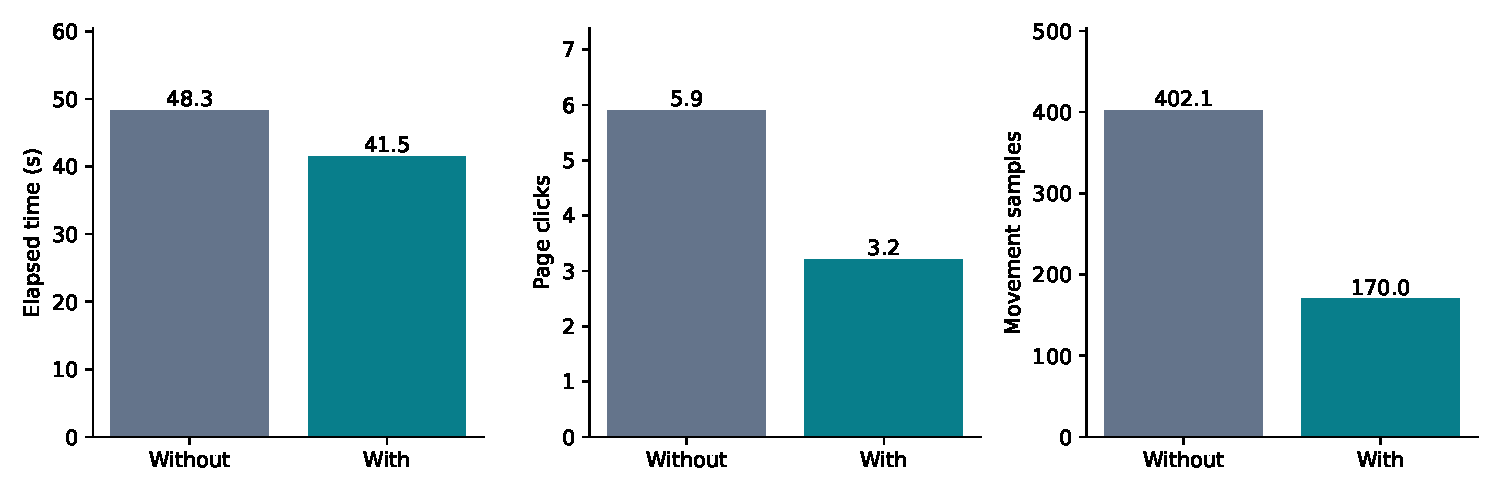
\includegraphics[width=\linewidth]{expanded.pdf}
\caption{Recorded data means for elapsed time, page clicks and movement samples. Each panel uses its own units; bars do not represent uncertainty.}\label{fig:Recorded}
\end{figure}

Across all 30 sessions, mean elapsed time was 48.31 seconds without assistance and 41.46 seconds with assistance, a 14.2\% reduction. Mean page clicks decreased from 5.87 to 3.16, a 46.2\% reduction and movement samples from 402.12 to 170.00, a 57.7\% reduction . Pointer distance fell from 7,155.0 to
2,187.72 pixels. These observations support lower recorded navigation effort with assistance; they do not isolate its causal contribution from practice.

\subsection{Task-specific outcomes}
Table~\ref{tab:tasks} shows that time benefits are not uniform. In the recordings, the outline task became faster, while the assignment task took longer with assistance. An overall average alone could suggest that assistance accelerated both tasks.
\begin{table}[htbp]\centering\small
\caption{Mean elapsed seconds by workflow; change is assisted minus unassisted time.}\label{tab:tasks}
\begin{tabular}{lrrr}\toprule
Dataset / task & Without & With & Change\\\midrule
Recorded sessions / outline & 61.82 & 36.81 & -25.01 \\
Recorded sessions / assignment & 34.81 & 46.11 & +11.30 \\


\bottomrule\end{tabular}\end{table}

Recorded success labels indicate 88.9\% tasks completed without assistance  and 100\% with assistance. Both labeled failures were unassisted outline tasks.

\subsection{Endpoint discrepancies and preliminary claims}
Of the seven recorded sessions that attempted outline first, four ended at a title other than Syllabus: P25 and P28 at Resources, P26 at course Overview, and P27 at Home Overview. This confirms the four-of-seven endpoint observation at the title level. However, P25 and P28 were marked successful. The guide notes that outline files may also be available through Resources. Without screen video or file-content evidence, these cases cannot be confidently reclassified as failures. We preserve the labels and disclose the discrepancy.

The preliminary claim of ten participants is not supported by ten direct recordings: nine are present. All nine recorded sessions took less time on their second unassisted task than their first unassisted task, but P20 and P21 attempted assignment first. This is not equivalent to saying assignment was always easier. The preliminary averages of approximately 58 and 32 seconds do not match the task means of 61.82 and 34.81 seconds. Approximate click and movement figures should likewise be replaced by Table~\ref{tab:results}. The supplied summary's description of 30 students mixes recording sources, and its headline values use medians of session averages rather than the means reported here.

\section{Analysis and Discussion}
\subsection{Navigation effort and elapsed time}
The strongest descriptive pattern is a reduction in navigation activity. Fewer clicks, shorter paths and fewer revisits are consistent with following a direct sequence instead of searching multiple locations. One-step presentation and pointing provide a plausible explanation, but the experiment did not isolate their individual contributions through component ablations.

Reduced navigation activity is not a proportional reduction in elapsed time. In the recordings, the assistant occupied an average of 31.88 seconds per assisted task. Time excluding those turns was only 9.70 seconds, but the participant experienced the full 41.57-second duration. Omitting speech and waiting would exaggerate practical speed benefits. Figure~\ref{fig:tasktime} shows the task-dependent tradeoff.
\begin{figure}[htbp]\centering
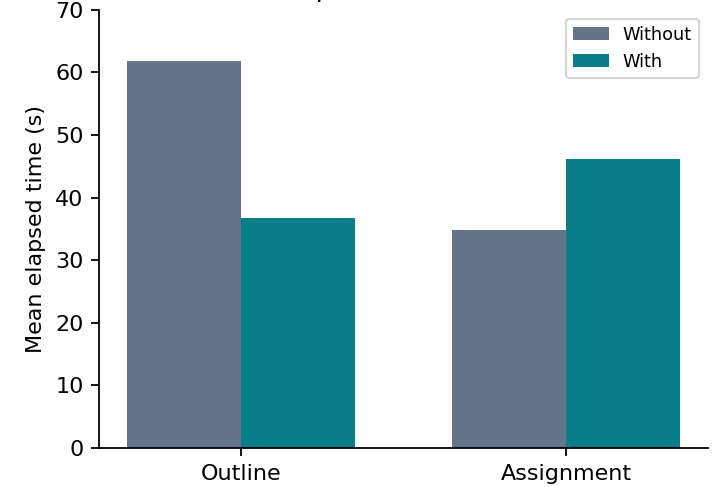
\includegraphics[width=\linewidth]{task_time_1.png}
\caption{Task-specific elapsed time in the recorded dataset. Repetition and assistant overhead affect interpretation.}\label{fig:tasktime}
\end{figure}

\subsection{Familiarity, order and interpretation}
Participants generally encountered assisted tasks after unassisted attempts. The seven later recorded sessions also put outline first and assignment second. Later improvements can reflect knowledge of course tabs and LMS layout acquired during the preceding attempt, even without assistance. Task difficulty provides another explanation. Neither mechanism can be separated by the current design.

\begin{table}[htbp]\centering\small
\caption{Interpretation of findings and alternative explanations.}\label{tab:interpret}
\begin{tabularx}{\linewidth}{>{\raggedright\arraybackslash}X>{\raggedright\arraybackslash}X>{\raggedright\arraybackslash}X}\toprule
Observation & Supported interpretation & Unresolved explanation\\\midrule
Lower click and movement means & Guidance is associated with more economical routes & Practice, repetition and generation assumptions affect pooled results\\
Faster outline, slower assignment & Assistance has a task-dependent time tradeoff & Instruction length and familiarity were not independently manipulated\\
Four non-Syllabus endpoints & Some users stopped at potentially unexpected locations & Resources may contain a valid outline\\
Higher labeled completion & All assisted recorded tasks received positive labels & Small sample and inconsistent endpoints limit inference\\
Second unassisted task faster & Consistent within-session sequence pattern & Task identity and order are intertwined\\\bottomrule
\end{tabularx}\end{table}

Table~\ref{tab:interpret} separates behavior from possible causes. P20 is only one assistant-first recording, insufficient to resolve the order effect. A stronger follow-up should balance condition and workflow order, use comparable tasks that have not just been completed, and define an auditable success criterion. Different-course repetitions should be documented consistently rather than inferred from a changing protocol.

\subsection{What the evaluation establishes}
The results are consistent with the problem statement: finding a destination can require considerable exploration even when the task is simple. They support the feasibility of contextual instructions alongside an application. The dataset tests the analysis pipeline across more trajectories, but its generated records cannot independently validate user behavior or compensate for the small observed sample.

The absence of retained feedback prevents a claim that participants preferred the assistant or felt less frustrated. Voice and text are implemented options, but the study does not establish outcomes for users with specific disabilities. A11yNav is a working guided-navigation prototype with encouraging behavioral evidence and identifiable performance costs.

\section{Challenges and Limitations}
\subsection{Documentation and coverage}
The team reports that the LMS lacked a structured document mapping its interface and workflows. The project authored its own guides, with feature names, ordered steps and target metadata. This makes retrieval useful but creates a maintenance obligation: changed labels, permissions or course layouts can invalidate a guide. Live-check notes document individual checks, not continuing correctness after future LMS changes.

Most external applications do not provide workflows in this format. Supporting Microsoft 365 or Blender requires additional documentation, target-location logic, testing and possibly new integration mechanisms. Browser and demonstration-shop guides illustrate extensibility, but do not establish arbitrary-application coverage.

\subsection{Voice recognition and reliability}
The team reports accent-recognition difficulties with Whisper. Vocabulary prompting, English transcription settings, final voice-activity filtering, hosted transcription and typed-input fallback are concrete implementation responses. Their effectiveness against particular accents was not measured. They are mitigations rather than a demonstrated solution.

Visual localization depends on screenshot readability, backend availability and model accuracy. Accessibility-tree inspection can fail when controls are missing or hidden. Bounded fallback addresses some failures, while permissive progression can introduce false completion. Correctly locating a button does not establish that its use achieved the intended outcome.

Historical tests record inference delays and rejected actions in the search demonstration. Tests using fake models validate application logic but do not prove live model reliability. No fresh application regression run was performed for this report, and historical test counts are not current suite results.

\subsection{Experimental limits}
The human evidence consists of nine sessions, two task types and one LMS setting. Prior experience and participant characteristics are undocumented. Order, repetition and procedural changes limit causal attribution. Expansion provides records rather than additional independent participants. Success labels have unresolved endpoint discrepancies. Mouse metrics depend on recording and device characteristics, and pauses may represent reading or waiting rather than confusion. Runtime backend choices, qualitative feedback, long-term learning and independent final-state validation are absent.

\section{Conclusion}
A11yNav addresses the difficulty of finding and following procedures in unfamiliar interfaces. It combines curated guide retrieval, step-by-step text and speech, accessibility-tree inspection and bounded visual localization. Users retain control of LMS actions while the assistant maintains context and provides specific recovery behavior.

The evaluation covers two Sakai workflows under assisted and unassisted conditions. The analysis includes 30 sessions providing the human validation comparison. Recorded data show lower click and movement counts, a modest overall elapsed-time reduction, and positive facilitator labels for all assisted tasks. The assignment task nevertheless took longer with assistance, and assistant interaction time was substantial.

The project achieved a working implementation and preliminary behavioral evaluation. It did not establish a general causal improvement across applications. Priorities are stronger final-state verification, shorter assistance overhead, consistent outcome criteria, retained feedback and a balanced study with additional independent participants. Guided navigation offers a promising way to bring application knowledge to the moment of use, provided its benefits are evaluated alongside its costs and failure modes.

\clearpage\addcontentsline{toc}{section}{References}
\begin{thebibliography}{9}
\bibitem{nielsen} J. Nielsen. \emph{10 Usability Heuristics for User Interface Design}. Nielsen Norman Group. \url{https://www.nngroup.com/articles/ten-usability-heuristics/}.
\bibitem{lewis} P. Lewis et al. \emph{Retrieval-Augmented Generation for Knowledge-Intensive NLP Tasks}. 2020. arXiv:2005.11401. \url{https://arxiv.org/abs/2005.11401}.
\bibitem{radford} A. Radford et al. \emph{Robust Speech Recognition via Large-Scale Weak Supervision}. Proceedings of Machine Learning Research, vol. 202, 2023. \url{https://proceedings.mlr.press/v202/radford23a.html}.
\bibitem{project} A. S. Babar, G. Khatwani and I. I. Nazar. \emph{A11yNav project source, study protocol and experiment records}. Local project snapshot inspected for this report. \url{https://github.com/Ibrahim-1rfan/A11yNav}. Primary evidence: \texttt{src/cua/}, \texttt{knowledge/lms/}, \texttt{study/STUDY\_DAY.md}, and \texttt{analysis/analysis/}. Accompanying support files document recomputation.
\end{thebibliography}
\end{document}

